% This came from my ECE528 repo, check there if you need to add something
\documentclass[11pt]{article}

\usepackage{sectsty}
\usepackage{graphicx}
\usepackage{amsfonts}
\usepackage{amssymb}
\usepackage[]{amsmath}

% Margins
\topmargin=-0.45in
\evensidemargin=0in
\oddsidemargin=0in
\textwidth=6.5in
\textheight=9.0in
\headsep=0.25in

\title{ECE 498: Trust in Critical Infrastructure HW1}
\author{Eric Silk}
\date{\today}

\newcommand{\qed}{\hfill$\square$}

\begin{document}
\maketitle
\pagebreak

%--Paper--

\section*{Problem 1}
\subsection*{Statement}
Consider a figure illustrating a water tank:

\begin{figure}[h]
    \begin{center}
        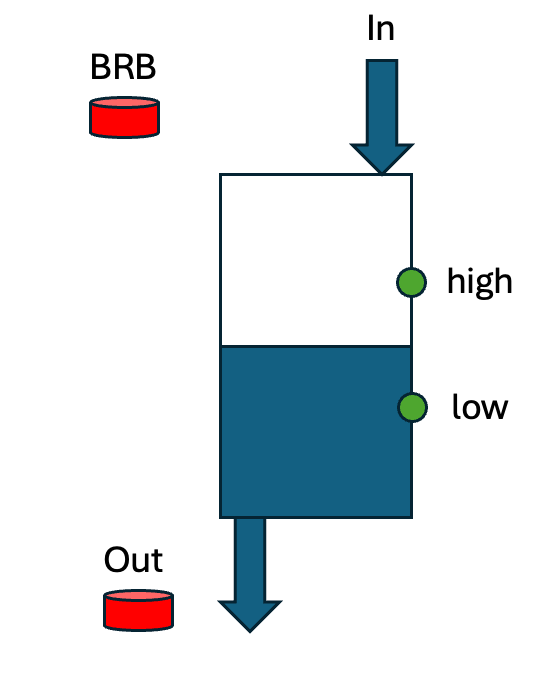
\includegraphics[width=0.5\textwidth]{water_tank.png}
    \end{center}
\end{figure}

\noindent
It has a valve "In" which when open allows a flow of water to enter the tank. It
has a value "Out" which when open allows water that is in the tank to drain out.
A sensor "high" has value true of the tank's water level has reached its
position, and a sensor "low" which has value true if the tank's water level is
at least as high as its position. An input BRB ("Big Red Button") when true
allows the In value to be open, and an input "Out" when true allows the valve
Out to be open. However, if the water has reached the level of sensor "high" the
"In" value is turned off, and if the water level drops below the sensor "low"
the "Out" sensor is turned off.

Prepare for class on Sept 16 for presentation/discussion

\begin{enumerate}
    \item Define Boolean variables for the inputs, sensors, and valves, and give
          a Boolean equation for the state of each valve, as a function of the inputs
          and sensors.
    \item Draw a Ladder Logic diagram for a PLC that would control this tank,
          according to these rules
    \item Write an equivalent Instruction List program for a PLC, using syntax
          which is in accordance with specifications of IEC 61131-3.
    \item (Submit by Sept 23) Implement either solution in openPLC
\end{enumerate}

\pagebreak
\subsection*{Solution}
\subsubsection*{Truth Table}
\begin{table}[h!]
    \begin{tabular}{llll|lll}
        \multicolumn{4}{c|}{\textbf{Inputs}} & \multicolumn{3}{c}{\textbf{Outputs}}                                                                       \\
        Big Red Button                       & Out                                  & High Water Sensor & Low Water Sensor & Water In & Water Out & Error \\ \hline
        0                                    & 0                                    & 0                 & 0                & 0        & 0         & 0     \\
        0                                    & 0                                    & 0                 & 1                & 0        & 0         & 0     \\
        0                                    & 0                                    & 1                 & 0                & 0        & 0         & 1     \\
        0                                    & 0                                    & 1                 & 1                & 0        & 0         & 0     \\
        0                                    & 1                                    & 0                 & 0                & 0        & 0         & 0     \\
        0                                    & 1                                    & 0                 & 1                & 0        & 1         & 0     \\
        0                                    & 1                                    & 1                 & 0                & 0        & 0         & 1     \\
        0                                    & 1                                    & 1                 & 1                & 0        & 1         & 0     \\
        1                                    & 0                                    & 0                 & 0                & 1        & 0         & 0     \\
        1                                    & 0                                    & 0                 & 1                & 1        & 0         & 0     \\
        1                                    & 0                                    & 1                 & 0                & 0        & 0         & 1     \\
        1                                    & 0                                    & 1                 & 1                & 0        & 0         & 0     \\
        1                                    & 1                                    & 0                 & 0                & 1        & 0         & 0     \\
        1                                    & 1                                    & 0                 & 1                & 1        & 1         & 0     \\
        1                                    & 1                                    & 1                 & 0                & 0        & 1         & 1     \\
        1                                    & 1                                    & 1                 & 1                & 0        & 1         & 0
    \end{tabular}
\end{table}

Let $I$ indicate inputs and $O$ indicate outputs, using descriptive subscripts.

\begin{equation}
    O_{error} \equiv I_{high} \land \lnot I_{low}
\end{equation}
\begin{equation}
    O_{in} \equiv I_{brb} \land \lnot I_{high} \land \lnot O_{error}
\end{equation}
\begin{equation}
    O_{out} \equiv I_{out} \land I_{low} \land \lnot O_{error}
\end{equation}

\end{document}